%
% SECCI��N: INTRODUCCION A PUNTEROS
%

\section{Introducci�n}

\subsection{�Qu� es un puntero?}

Podr�amos imaginar un puntero como una \emph{flecha} que apunta a otra
variable, pero esto es s�lo para aclararnos a la hora de hacer
esquemas. En realidad, dentro del ordenador, una variable puntero no
es m�s que una direcci�n de memoria, un puntero nos dice
\textbf{d�nde} se encuentra almacenado el valor de la variable a la que apunta. Si
nos quedamos con esta �ltima definici�n (la de direcci�n de memoria),
nos ser� m�s f�cil aclararnos cuando trabajemos con punteros a gran
escala.\\

Como ya sabemos, al declarar una variable lo que estamos haciendo es
\emph{reservar} espacio en memoria para esa variable (el tama�o del
espacio reservado depender� del \emph{tipo} de la variable). Pues
bien, al declarar un puntero lo que hacemos es reservar espacio para
almacenar \emph{una direcci�n de memoria}, no el contenido de la
variable.\\

La siguiente figura muestra tres variables, de tipos \verb+char+, \verb+int+ y
\verb+double+, y un puntero a cada una de ellas:

\begin{figure}[H]
\begin{centering}
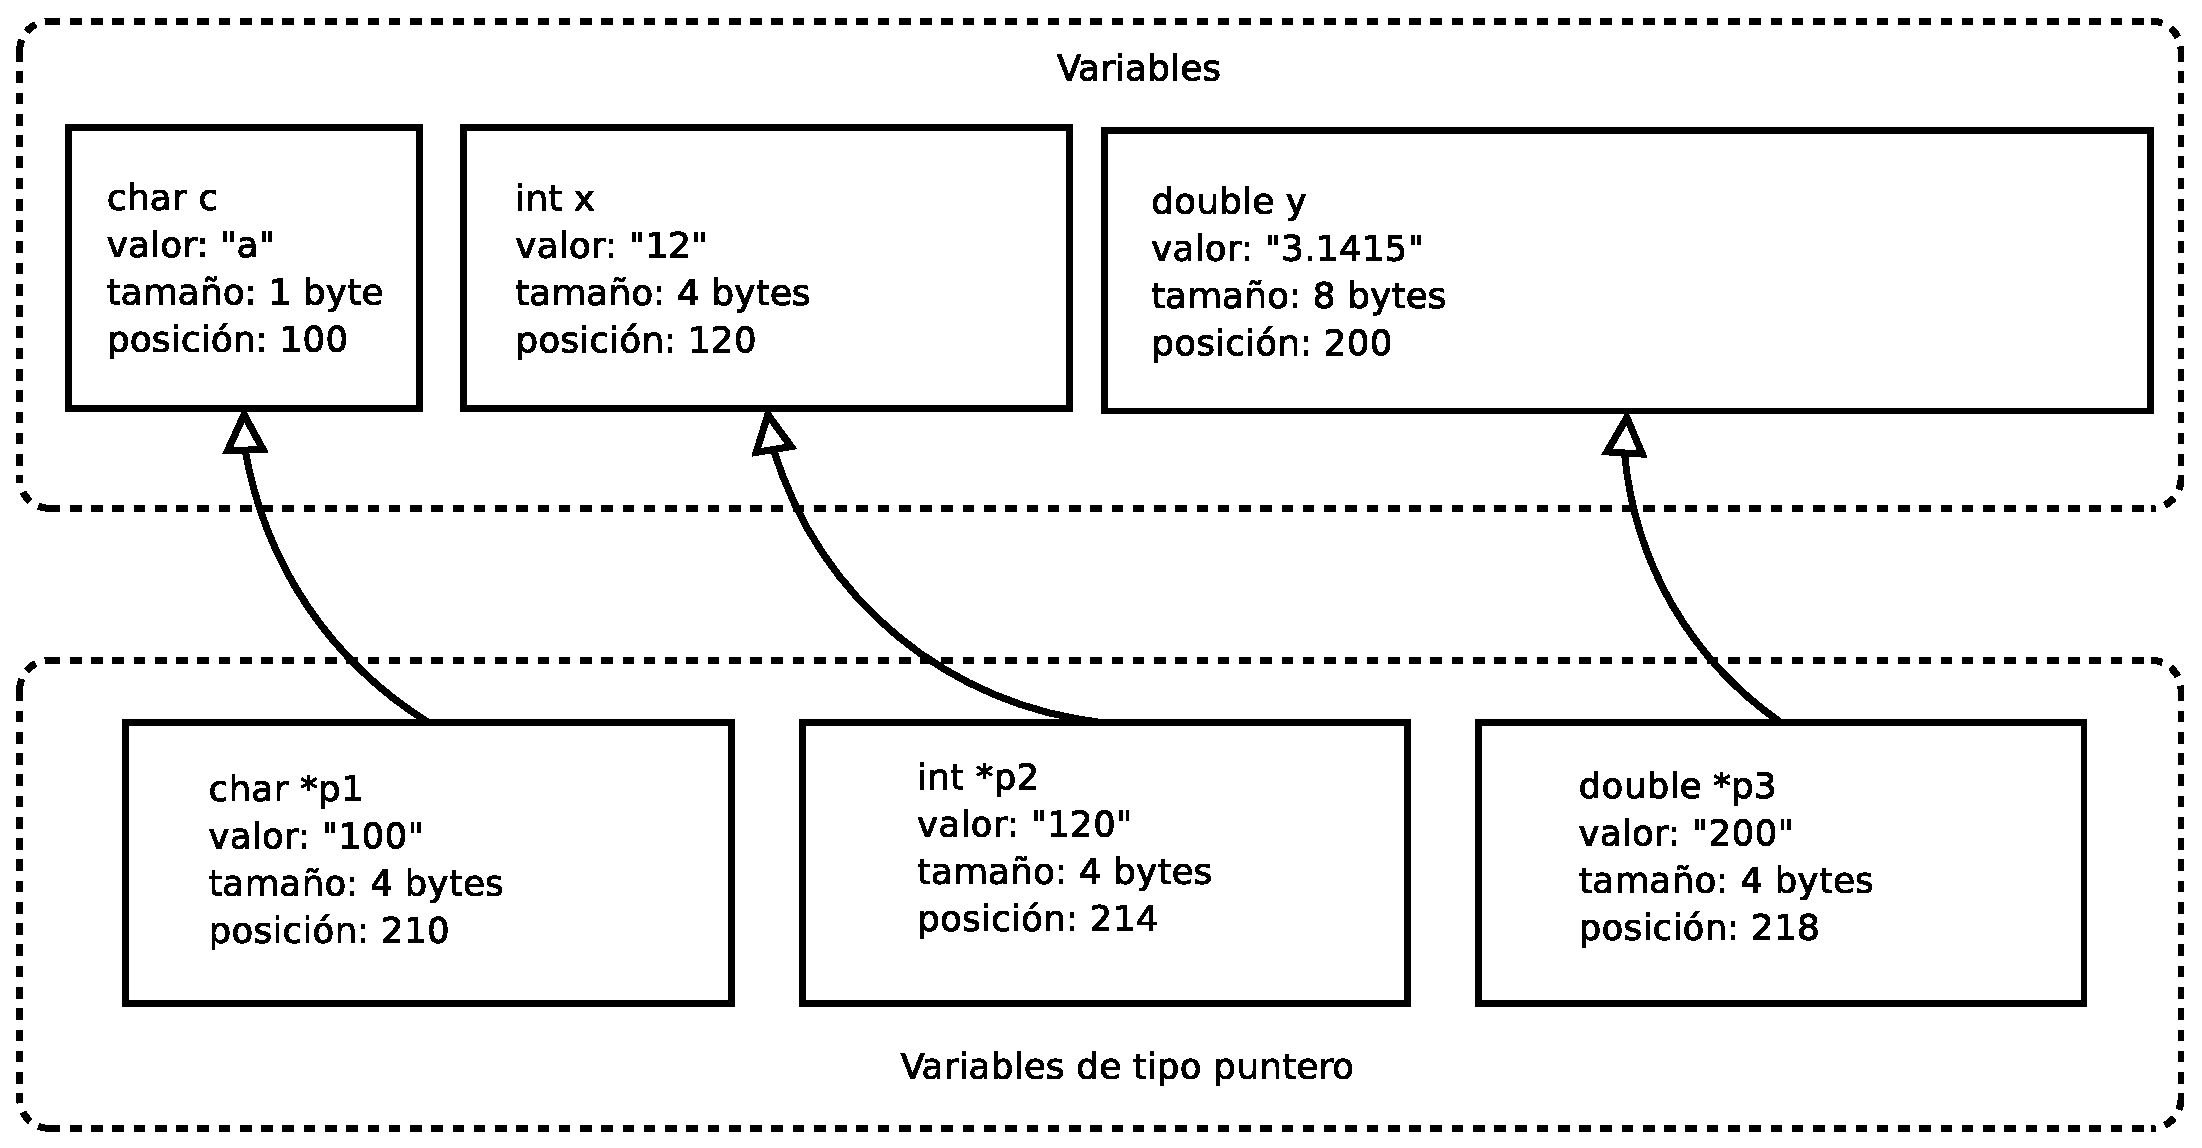
\includegraphics[width=180mm]{punteros/images/general.eps}
\caption{Punteros a variables \texttt{char}, \texttt{int} y \texttt{double}}
\end{centering}
\end{figure}

Tomemos como ejemplo la variable de tipo \verb+char+. Est� almacenada en la
direcci�n de memoria (fict�cia) 100. El contenido de dicha posici�n
(esto es, el contenido de la variable) es el car�cter ``a''. Por otro
lado, el puntero p1 se encuentra en la direcci�n 210, y su valor es
100. Como vemos, el contenido de la variable p1 (puntero) es la
direcci�n de la variable \verb+char+.\\

Como se ve en la figura, mientras que el tama�o que ocupan en memoria
las variables es distinto (un \verb+char+ ocupa un byte, un double ocupa 8
bytes), el tama�o que ocupan las variables tipo puntero es siempre el
mismo: 4 bytes. Esto es l�gico: las direcciones de memoria siempre
ocupan el mismo tama�o. \footnote{Es importante recordar que los 
tama�os de las variables \texttt{char}, \texttt{int} y \texttt{double} aqu� especificados son 
dependientes de la plataforma.} 

\subsection{�Para qu� necesito yo un puntero?}

Es posible que al abordar un concepto algo m�s abstracto que los
que surgen al aprender un lenguaje de programaci�n, sea dif�cil
imaginar para qu� sirve. Al plantearnos esa pregunta, surgen dos
respuestas inmediatas:

\begin{itemize}
\item para poder usar ``memoria din�mica''.
\item para poder usar ``argumentos por referencia''.
\end{itemize}

Ambos conceptos van a ser tratados con m�s profundidad en las
secciones \ref{mem_dinamica} y \ref{valor_vs_referencia}.

